\documentclass{article}
\usepackage{tikz}
\usetikzlibrary{shapes.geometric, arrows, positioning, calc}

\begin{document}

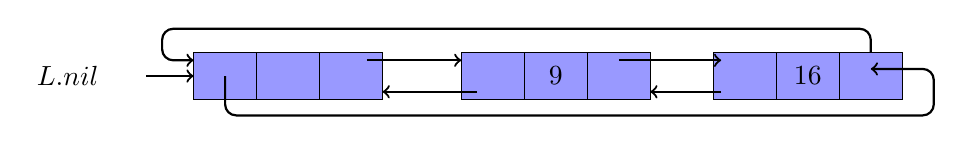
\begin{tikzpicture}
    % L.nil node
    \node at (-2, 0) {$L.nil$};
    
    % Blue rectangle nodes
    \node[text =black,rectangle, draw, minimum width=0.8cm, minimum height=0.6cm, fill=blue!40] (1) at (0, 0) {};
    \node[text =black,rectangle, draw, minimum width=0.8cm, minimum height=0.6cm, fill=blue!40] (2) at (0.8, 0) {};
    \node[text =white,rectangle, draw, minimum width=0.8cm, minimum height=0.6cm, fill=blue!40] (3) at (1.6, 0) {};
    \node[text =black,rectangle, draw, minimum width=0.8cm, minimum height=0.6cm, fill=blue!40] (4) at (3.4, 0) {};
    \node[text =black,rectangle, draw, minimum width=0.8cm, minimum height=0.6cm, fill=blue!40] (5) at (4.2, 0) {9};
    \node[text =white,rectangle, draw, minimum width=0.8cm, minimum height=0.6cm, fill=blue!40] (6) at (5, 0) {};
    
    \node[text =black,rectangle, draw, minimum width=0.8cm, minimum height=0.6cm, fill=blue!40] (7) at (6.6, 0) {};
    \node[text =black,rectangle, draw, minimum width=0.8cm, minimum height=0.6cm, fill=blue!40] (8) at (7.4, 0) {16};
    \node[text =white,rectangle, draw, minimum width=0.8cm, minimum height=0.6cm, fill=blue!40] (9) at (8.2, 0) {};
    
    % Connections
    \draw[->,thick] (-1,0) to (-0.4,0);
   \draw[->, thick,rounded corners] (8.2,0.3) to (8.2,0.6)to (-0.8,0.6) to (-0.8,0.2) to (-0.4,0.2);
\draw[->, thick,rounded corners] (0,0) to (0,-0.5) to (9,-0.5) to(9,0.09) to (8.2,0.09);
\draw[->,thick] (1.8,0.2) to (3,0.2);
\draw[->,thick] (3.2,-0.2) to (2,-0.2);
\draw[->,thick] (5,0.2) to (6.3,0.2);
\draw[->,thick] (6.3,-0.2) to (5.4,-0.2);
\end{tikzpicture}

\end{document}
